\subsection{Provenance Image Filtering}
\label{sec:prop:filtering}
The problem of image filtering for the provenance task is different from the typical image retrieval task: a given query image may %simultaneously
fulfill one or both of the following conditions:

\begin{itemize}
    \item The query may have a relationship to various \emph{near duplicates}. The near duplicates may be \emph{hosts} of the query (in the case of the query being a composite that inherits the background from a near duplicate) or the query itself may be a host, as in the case of the query donating a background to the near duplicates.
    
    \item The query may be a composite with a relationship to one or more donors, whose content may be entirely disjoint.
    Donors can even be composites themselves, with their own hosts and donors.
\end{itemize}

In such scenarios, the retrieval method must return as many of the directly and transitively related images as possible.
These aspects define a unique image retrieval and filtering problem, known as \emph{Provenance Image Filtering}~\cite{pinto2017filtering, nist2017plan}, which is different from more typical \emph{near-duplicate} or \emph{semantically similar} image retrieval.
%Therefore, a new system must be designed with the specific purpose of solving such a task.
In this work, we assume that a ground-up system must be deployed for search, retrieval, and filtering, instead of relying on currently available resources such as \emph{Google}~\cite{barroso2003web} or \emph{TinEye}~\cite{jacquicheng}.
%As depicted in Fig.~\ref{fig:solution}, the proposed system starts with a modified interest point selection method (detailed in %Sec.~\ref{sec:prop_spread_kp}), whose output is fed to %a highly-parallelizable
%an image index computation approach inspired by the work in~\cite{johnson2017billion} (detailed in Sec.~\ref{sec:prop_indxing}).
%Once the image indices are obtained, the image search is performed in a way close to~\cite{johnson2017billion} (which is explained in %Sec.~\ref{sec:prop_search}), with the additional step of \emph{iterative filtering} (explained in %Sec.~\ref{sec:prop_iterative_filtering}) that adapts image filtering to the provenance scenario.
%Finally, in Sec.~\ref{sec:prop_scaling}, we explain the strategy to handle millions of images.
 
\vspace{0.2cm} 
\subsubsection{Distributed Interest Point Selection} 
\label{sec:prop_spread_kp}
Due to the nature of the manipulations seen in tampered images, it is important to build a filtering system that is tolerant to a wide range of image transformations.
Hence, we adopt a low-level image representation that is based on interest points and local features, since they are reportedly tolerant to transformations such as scaling, rotation, and contrast adjustment~\cite{Bay:CVIU:2008}.
Nevertheless, while regular interest points are mostly designed to identify corners and blobs on the image, we also want to describe and further index homogeneous areas with low response and consequently a sparse amount of detected interest points, for retrieving images with the same type of content.
Although one can use a dense sampling approach to extract interest points within those regions, this is computationally prohibitive in the context of searching millions of images~\cite{pinto2017filtering}.

Therefore, we introduce a new method called \emph{distributed interest point selection} that aims at keeping a sparse approach while being able to provide interest points inside low-response areas.
For that, we extend Hessian-based detectors (such as Speeded-Up Robust Features (SURF)~\cite{Bay:CVIU:2008}) in the following way.
Instead of employing a threshold $t$ to collect interest points whose local Hessian values are greater than $t$, we define a parameter $p$ that expresses the fixed amount of interest points we want to extract from each target image.
Within these $p$ interest points, $m < p$ interest points are extracted for the reason of being the top-$m$ regions with the $m$ strongest Hessian values.
The remaining $n = p - m$ are extracted from the set containing the post-top-$m$ interest points, which is also sorted according to the Hessian response.
Starting from the $(m+1)$-th strongest interest point, we only add the current interest point if it does not \emph{overlap} with another already selected interest point; otherwise, we try to add the next strongest interest point, up to the point of obtaining $n$ interest points.

\begin{figure}[!t]
\centerline{
    \subfloat[]{\frame{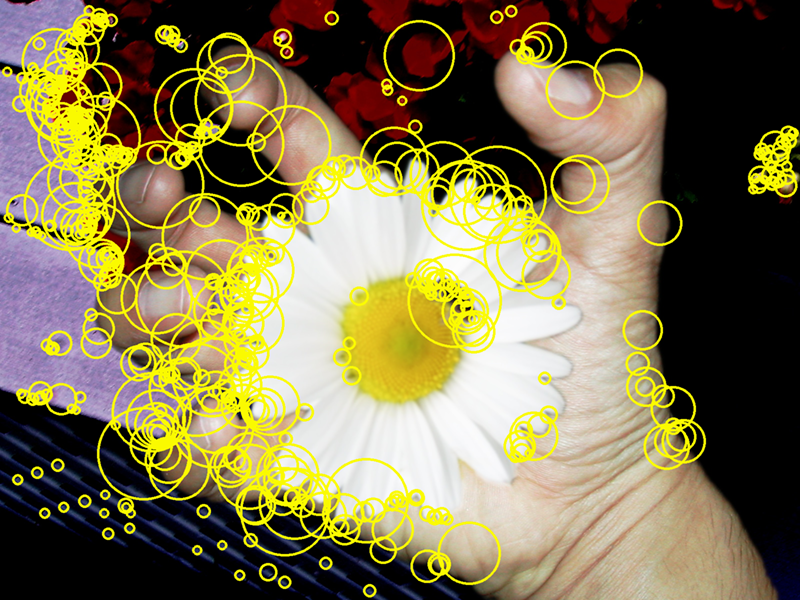
\includegraphics[width=4cm]{figures/rsurf.png}}}
    \hfil
    \subfloat[]{\frame{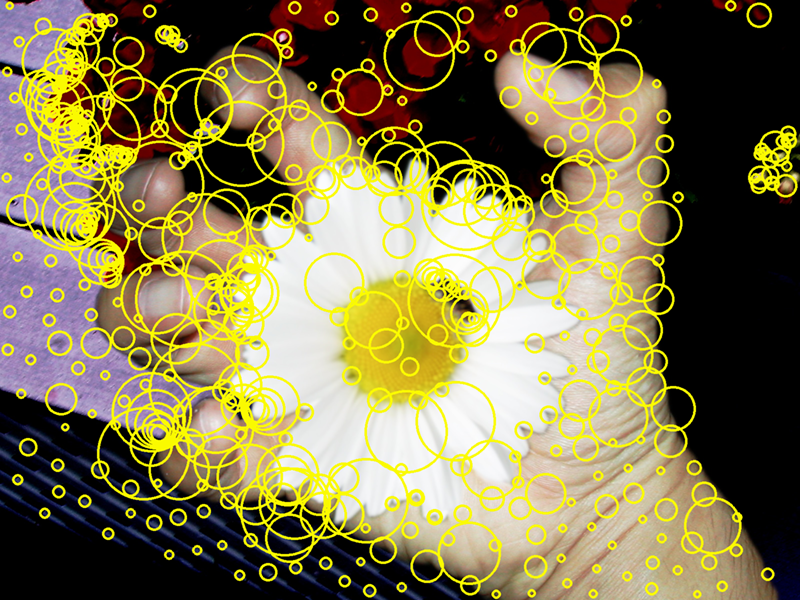
\includegraphics[width=4cm]{figures/dsurf.png}}}
}
\caption{Effects of using the approach of distributed interest point selection.
In (a), the result of a regular SURF interest point detection.
In (b), the result of the distributed approach over the same image, with many more points over homogeneous regions, such as the skin of the wrist.}
\label{fig:disitributed_kp}
\end{figure}

Fig.~\ref{fig:disitributed_kp} depicts the effect of using the distributed approach along with SURF.
Fig.~\ref{fig:disitributed_kp}~(a) depicts a regular SURF detection, while Fig.~\ref{fig:disitributed_kp}~(b) depicts the distributed version, over the same image.
Fig.~\ref{fig:disitributed_kp}~(b) presents more points over the skin of the wrist and background (which are more homogeneous regions) than Fig.~\ref{fig:disitributed_kp}~(a).

%Taking into consideration that each interest point is actually a circular blob with a center $(x, y)$ and a radius $r$, we establish that two points overlap if they do not collide (\textit{i.e.}, they do not share describable content).

\vspace{0.2cm} 
\subsubsection{\RED{Database Indexing}}
\label{sec:prop_indxing}
\RED{The next step is to build the image index structure. %, which we refer to as the CBIR system.
After interest point detection and feature extraction, we are left with $p$ description vectors per image.
For an image collection $C$:}

\begin{equation}
C_i \in C, \quad s.t.\quad  i \in \mathcal{I}_{img} = \{0, 1, \ldots, |C|\},
\end{equation}

\noindent \RED{our subsequent feature collection $F$ is:}

\begin{equation}
F_i \in F, \quad s.t.\quad  i \in \mathcal{I}_{ind} = \{0, 1, \ldots, |C| \times p\},
\end{equation}

\noindent \RED{where $\mathcal{I}_{img}$ denotes the numbered index set of full images within $C$, and $\mathcal{I}_{ind}$ indicates the subsequent numbered index set assigned to individual features in $F$.
We transform $F$ to a new space using \emph{Optimized Product Quantization} (OPQ)~\cite{ge2013optimized} to make the feature space well-posed for coarse \emph{Product Quantization} (PQ).
We refer to this new rotated feature set as $F_{r}$.
From a random sample of $F_{r}$, a coarse set of representative centroids $O$ is generated using PQ.
A subsequent \emph{Inverted File System with Asymmetric Distance Computation} (IVFADC)~\cite{Jegou:TPAMI:2011}) is generated from $O$, allowing for fast and efficient search.}

\vspace{0.2cm} 
\subsubsection{\RED{Image Search}} % and Retrieval}
\label{sec:prop_search}
%Once the CBIR system is built, it can be searched via feature-wise queries.
\RED{Once the database images are indexed, a search procedure can be performed via feature-wise queries.
For a query image $Q$, a set of $p$ distributed SURF features $F_{d}$ is extracted, rotated according to $F_{r}$, and submitted to the system.
Each image $Q$ leads to a matrix of indices of \emph{Approximate Nearest Neighbors} (ANN) $R$ of size $|F_{d}| \times K$, where $K$ is the parameter of the $K$-nearest neighbors for the system to return.
Each $R_{ij}$ value of $R$ is computed using \emph{Asymmetric Distance Computation} (ADC)~\cite{Jegou:TPAMI:2011}:}
\vspace{-0.2cm} 

\begin{equation}
R_{ij}=\mathcal{S}(F_{d_{i}})_{j},\ s.t. \ i \in \{1,...,|F_{d}|\}\ \text{and}\  j \in \{1,...,K\}\,
\end{equation}

\noindent \RED{where $\mathcal{S}$ signifies a feature-wise query search on the IVFADC filtering system, $i$ denotes the $i$-th query feature of $Q$, and $j$ denotes the $j$-th ANN index of the $j$-th nearest feature belonging to $F_{r}$.
As a consequence, each row of $R$ corresponds to a feature in $F_{d}$, containing the $K$-nearest neighbor features, which we may consider as matched features.
We then map $R$ from the $\mathcal{I}_{ind}$ space to the $\mathcal{I}_{img}$ space.
The set of unique related image indices is computed as:}

%\begin{equation}
%\begin{aligned}
%& R_{i,j}=\mathcal{S}(F_{d_{i}})_{j},\ s.t.\\
%& i \in \{0,1,\ldots,|F_{d}|\}\ \text{and}\  j \in K,
%\end{aligned}
%\end{equation}

%\noindent \RED{where $\mathcal{S}$ signifies a single search query on the %CBIR
%filtering system, and $K$ is the parameter of the $K$-nearest neighbors for %the CBIR
%the system to return.
%The set $R$ is subsequently a matrix of size $|F_{d}|*K$, where each row corresponds to a feature in $F_{d}$, containing K nearest neighbor features. We then map $R$ from the $\mathcal{I}_{ind}$ space to the $\mathcal{I}_{img}$ space.
%As a consequence, each row of $R$ corresponds to a feature in $F_{d}$, containing $K$ nearest neighbor features.
%We then map $R$ from the $\mathcal{I}_{ind}$ space to the $\mathcal{I}_{img}$ space.
%The number of unique image indices is computed as:}

\begin{equation}
R_{img}=\mathcal{M}(R,\mathcal{I}_{ind},\mathcal{I}_{img}).
\end{equation}

\noindent \RED{where function $\mathcal{M}(R,\mathcal{I}_1,\mathcal{I}_2)$ maps index values in $R$ from the $\mathcal{I}_{ind}$ domain to the $\mathcal{I}_{img}$ index domain, allowing each $R_{ij}$ to represent the image it belongs to.
Once $R_{img}$ is obtained, a result set of images sorted by the number of matched features is calculated for giving the final global query results of $Q$.}

\RED{The score for each image indexed within $R_{img}$ is therefore denoted by ${freq}(x,R_{img})$, where $x \in \{R_{img}\}$ and ${freq}(x,\cdot)$ is a function that counts the number of occurrences of $x$.}

%The score for each value within ${R_{img}}$ is therefore denoted by the respective tally of feature-wise votes accumulated within $R$.
%Using this scheme, we are able to retrieve images that only partially match $Q$, even in the presence of noisy matches.
%Small local objects will have higher chances of receiving votes than spurious interest points, allowing for burstiness \cite{Jgou2009OnTB}.

%The score for each value within ${R_{img}}$ is denoted by:
%\begin{equation}
%    \mathcal{A}(x,R_{img}),
%\end{equation}

%\noindent where $\mathcal{A}(x,R)$ represents the accumulator that returns the tally of all values of $x$ within $R$.
% \begin{equation}
% \begin{aligned}
%     V_{i} =
%      \begin{cases} 
%       \underset{x \in \{R_{img}\}-V_{i-1}}{\operatorname{argmax}}\{\mathcal{A}(x,R_{img})\}, & \text{if  } i > 0 \\
%       \ \ \ \ \ \ \ \ 0, & \text{if  } i = 0 
%   \end{cases}
% \end{aligned}
% \end{equation}
%Using this scheme, we are able to retrieve images that only partially match $Q$, even in the presence of many noisy matches. Small local objects will have high chances of accumulating values, allowing for burstiness \cite{Jgou2009OnTB} while spurious interest points will not.

\vspace{0.2cm} 
\subsubsection{Iterative Filtering}
\label{sec:prop_iterative_filtering}
Once a first rank of images is retrieved through the search algorithm, we iteratively refine the results to add images that are not directly related to the query, but are still related in some way to its provenance.
%Refer to Fig.~\ref{fig:solution} for an illustration of this process.

In contrast to the approach described by Pinto et al.~\cite{pinto2017filtering}, which employs a two-tiered search to retrieve the small donors of the query after masking the regions that diverge between the query and the first images of the retrieved rank, in this work we employ the \emph{reciprocal condition matching measure} (RCMM) proposed in~\cite{brogan2017spotting} to identify and suppress the near duplicates of the query.
%Given that, the greater the RCMM between two images, the greater the possibility of them being near duplicates, we suppress the retrieved images whose RCMM values with the query are high.
Given that a large RCMM value between two arbitrary images indicates that they are probably near duplicates, we suppress the retrieved images whose RCMM values with the query are large.
% TODO: Daniel: ask Joel more details about this suppression. Is it based on a threshold? Maybe rank position?
The non-suppressed (and therefore non-near-duplicate) images of the current rank are then provided as new queries to the next search iteration, which is performed using the same method explained in Sec.~\ref{sec:prop_search}.

%By applying the above process for a number of iterations, we search various sets of non-near-duplicate queries (which are potentially donors) and end up with a set of ranks, which are then flattened and re-ranked using RCMM.
%In the end, we obtain a less query-centric rank of images, which contains the images directly and indirectly related to the query.
%As we show through experiments in Sec.~\ref{sec:results}, such a strategy improves the recall of the provenance image filtering task, when compared to the application of a regular CBIR system.

By applying the above process for a number of iterations, we search various sets of non-near-duplicate queries (which are potentially donors) and end up with a set of ranks, which are then flattened and re-ranked using RCMM.
In the end, we obtain a less query-centric rank of images, which contains not only images directly related to the query, but also transitively related (\textit{e.g.}, ancestors of the donors of the query).
As will be demonstrated in Sec.~\ref{sec:results}, such a strategy improves the recall of the provenance image filtering task.

% TODO: Daniel: Ask Joel to review the entire following section, including images.
% [MAJOR] Moved to the experimental setup >>>>>>>
%\vspace{0.2cm} 
%\subsubsection{Large-Scale Infrastructure}
%\label{sec:prop_scaling}
%
%Fig.~\ref{fig:filterPipeline} shows the proposed full pipeline for index \emph{training} and \emph{construction} (previously explained in Sec.~\ref{sec:prop_indxing}).
%Index training refers to the process of learning the OPQ rotations and PQ codebooks from a sampling of the local features that are extracted from the target dataset.
%We propose to perform such a step ahead of time with typical central processing units (CPU).
%Index construction, in turn, refers to the computation of the inverted file indices, after properly rotating the previously extracted local features.
%The learning of OPQ rotations and PQ codebooks can be done in advance on a CPU, but the construction of indices is well suited to the capabilities of graphical processing units (GPU), allowing for faster computation.
% TODO: Prof. Rocha's note: Clarify this last sentence. Make it clear what you did in CPU and in GPU.  
%
%\begin{figure}[t]
%\centering
%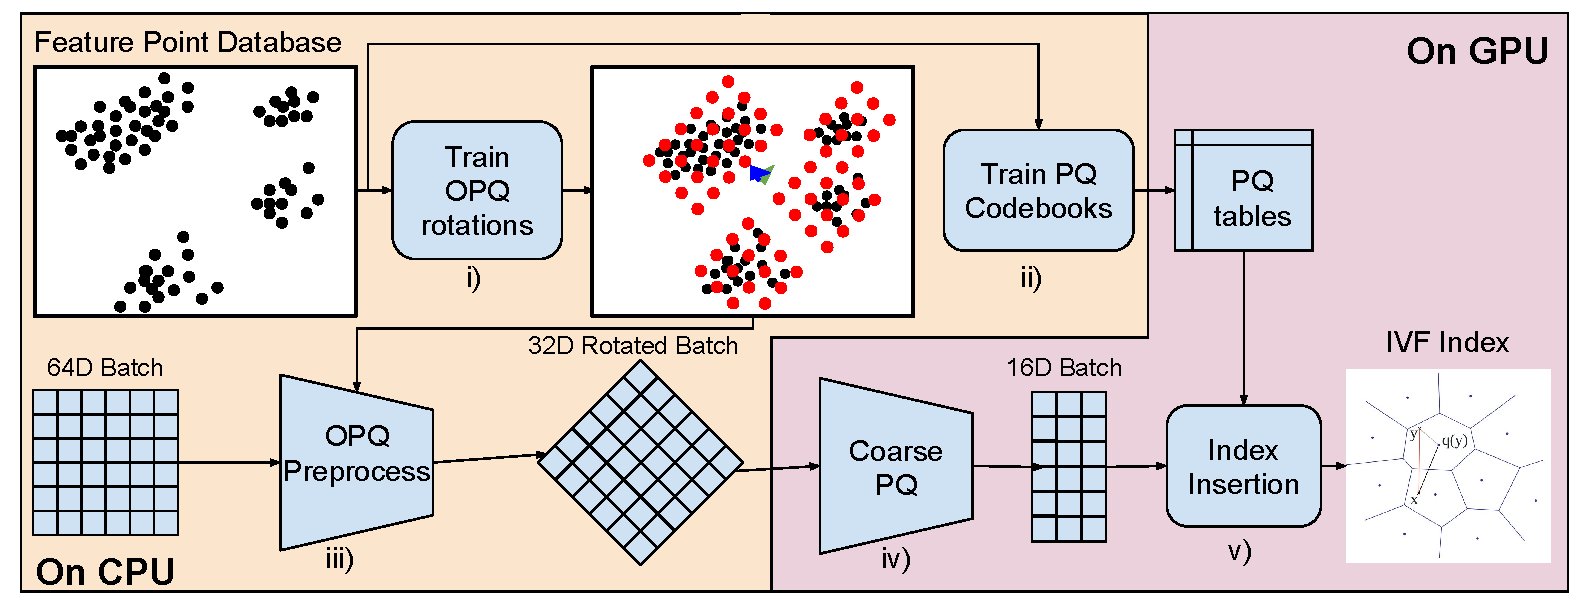
\includegraphics[width=9cm]{figures/Indexing_pipeline.pdf}
%\caption{Filtering pipeline infrastructure.
%The orange area (left) shows computations that are performed on a CPU.
%The purple area (right) shows the index ingestion steps that are performed on a GPU.}
%\label{fig:filterPipeline}
%\end{figure}
% TODO: Prof. Scheirer's note: make on CPU and on GPU labels bold.
%
%\begin{figure}[!htbp]
%\centering
%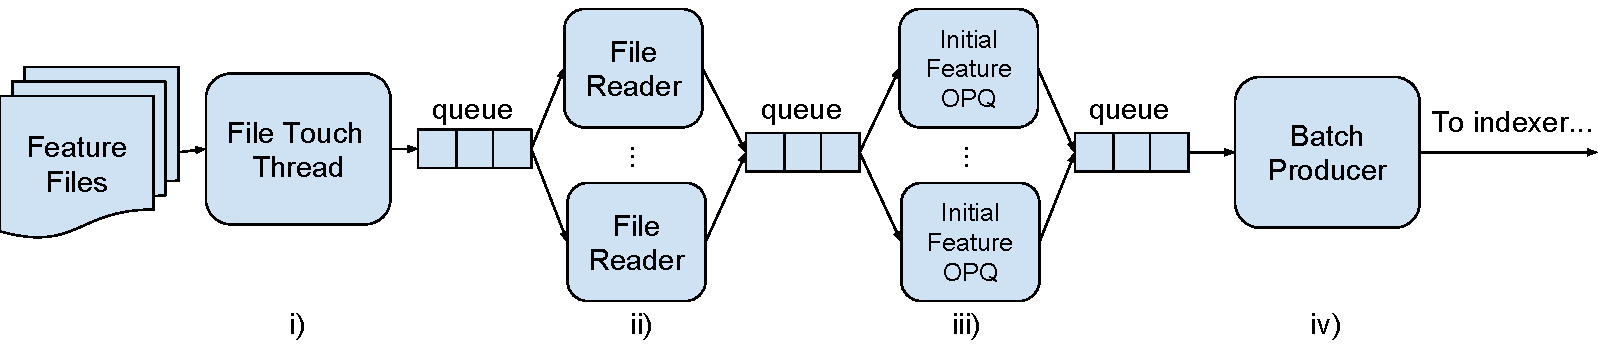
\includegraphics[width=9cm]{figures/Fileread_pipeline.pdf}
%\caption{
%Producer-consumer index ingestion.
%Each file contains features for an image.
%These file locations are pre-loaded into cache via a rate-limited ``touch" thread, and are read on a producer-consumer multi-threaded basis.}
%\label{fig:touchPipeline}
%\end{figure}
% TODO: Prof. Scheirer's note: make image texts larger.
%
%Besides employing GPUs to efficiently build and search an index of over 1 million high-resolution images, additional steps must be taken to increase the pipeline speed.
%To date, most indexing algorithms require singular large files containing all features to be ingested at once \cite{flann_pami_2014,Attach:binary_matching_crv2012}, either due to implementation choices or algorithm limitations.
%The operation of concatenating all features from a set of images into a single file is prohibitively time consuming when dealing with more than a few million interest points.
%Because our scenarios require the ingestion of multiple billions of interest points, a different solution must be adopted, in order to avoid the need for file concatenation.
%For that, we propose a multi-threaded producer-consumer setup, as shown in Fig.~\ref{fig:touchPipeline}.
%In our pipeline, we provide a single feature file per image.
%The pipeline begins with the ``touch" thread, which systematically loads image feature file locations into the computer's file system cache, for faster retrieval in later stages.
%Then, a reading thread takes touched files and loads them into memory.
%A third thread takes sets of loaded feature files and produces feature batches of size $B$ that are optimized in size for GPU ingestion.
%The fourth thread applies the initial OPQ pre-processing rotations to the feature set, before sending the final batch to the GPU. Using this method, we are able to process billions of features from high-resolution image datasets orders of magnitudes faster than previous methods.
% <<<<<<< [MAJOR] Moved to the experimental setup
